\subsection{Implementering}
I følgende afsnit vil den overordnede implementering af de enkelte dele blive beskrevet. Et overblik er givet i form af figur~\ref{fig:klientserver} hvor de primære komponenter er vist.

\begin{figure}
	\centering
	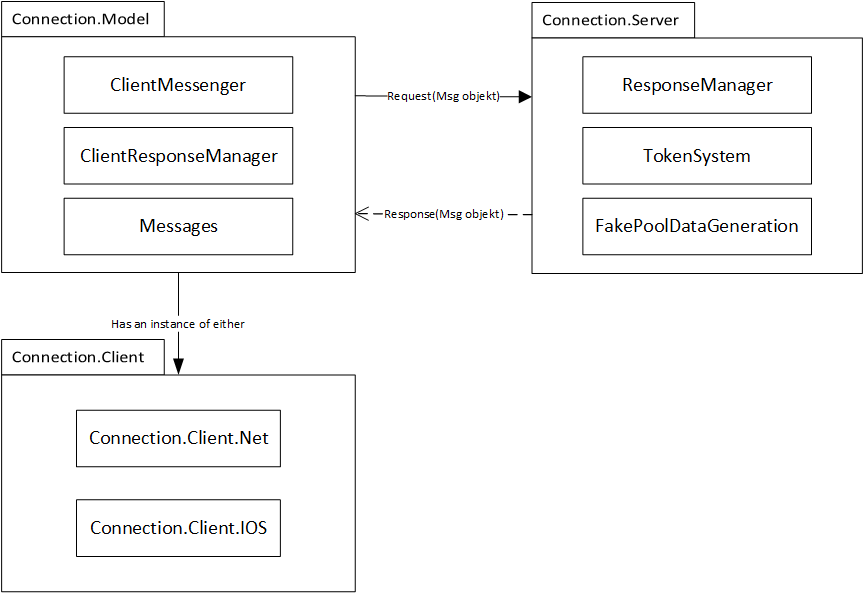
\includegraphics[width=0.7\linewidth]{figs/design/klientserver.PNG}
	\caption{Overblik over klient server struktur}
	\label{fig:klientserver}
\end{figure}

\subsubsection{Overordnet connection struktur}
\textit{Klient} delen består af et model projekt som er generelt for alle platforme, samt et klient projekt som er specifikt for hver platform. Dette er gjort for at gøre så meget som muligt anvendeligt på alle platforme. I model projektet er desuden defineret en række besked objekter, som anvendes ved kommunikation mellem klient og server.

\textit{Server} delen består af en række systemer, som tilsammen udgør en samlet server udviklet til at køre på en windows pc. Al kommunikation til databasen udgår fra serverdelen.

\subsubsection{Klient}
Klienten modtager besked objekter fra applikationslaget, og omdanner disse til en streng vha. json serializering. Strengen bliver sendt til serverdelen gennem en socket klient, der passer til den pågældende platform.
Klienten modtager derefter et svar fra serveren i form af et serialiseret besked objekt, som bliver deserialiseret til basis besked klassen. Denne indeholder en besked type, og klienten kan derefter deserialisere den modtagne streng til det korrekte besked objekt. Derefter bliver objektet sendt tilbage til applikationslaget. 

\subsubsection{Server}

Vedligeholder følgende funktioner i systemet.

\begin{itemize}
	\item Modtage, behandle og svare på requests fra klientdelen
	\item Varetage user sessions
	\item Kommunikere med databasen via metoder i databasedelen
	\item Simulere pool data
\end{itemize}

\subsubsection{Modtage, behandle og svare på requests fra klientdelen}
Serveren modtager via en Asyncronous Socket Client (ASC) en streng fra klientdelen. Denne bliver, som i klienten, lavet til et basis besked objekt. Denne bliver derefter behandlet vha. en switchcase, hvor der reageres på, hvilken message type, der er blevet sendt. Dette foregår i en ResponseManager klasse, og denne vil, i nogle situationer, være i stand til selv at udføre den kaldte request. Det gør den ved f.eks. at lave et kald til databasen og returnere svaret derfra.
I andre situationer, bliver kaldet sendt videre til en \textit{sub handler}, som f.eks. TokenMsgResponse, der tager sig af alle requests, som kræver at brugeren er logget ind. Dette er lavet således at ResponseManager checker, om brugeren er logget ind. Er dette tilfældet, bliver beskeden sendt videre til TokenMsgResponse. TokenMsgResponse behøver dermed ikke selv at kontrollere om brugeren er logget ind.
Hvis beskedtypen ikke genkendes, sendes svar tilbage til klienten om dette.

\subsubsection{User sessions}
For at holde styr på hvilke brugere, som er logget ind, er der udviklet et Token system. Dette system giver en øget sikkerhed, ved at brugeren kun sender password en enkelt gang, og det behøver derfor heller ikke at blive gemt i klienten. Desuden bliver der færre kald til databasen, da efterfølgende requests ikke behøver at kontrollere brugerens password via databasen.
Token systemet virker ved at en bruger, ved login, får tilknyttet en streng. Brugernavnet bliver, sammen med strengen og et timestamp, gemt i en klasse der hedder Token. Alle disse tokens bliver så vedligeholdt i en TokenKeeper. Når en bruger efterfølgende laver et request til serveren, sender klienten både username og token strengen med i sin request. Serveren kontrollerer derefter om dette stemmer overens med de data, som ligger i TokenKeeperen samt om det gemte timestamp er ældre end systemets valgte sessionstid.
En bruger kan godt være logget ind på flere enheder på samme tid. I det tilfælde vil hver enhed få tildelt en tokenstreng, og dermed har de ikke indflydelse på hinandens session.

\subsubsection{Kommunikere med databasen via metoder i database delen}
Serveren kommunikerer via tilgængelige metoder i systemets data-access layer. Dette beskriver i afsnittet om database og DAL.

\subsubsection{Simulerering af pool data}
Da Smartpool systemet ikke anvender reelle data, er der udviklet en FakePool klasse til at simulere dette. Denne opretter en af hver type sensor. Hver sensor bliver initieret med en værdi, der ligger indenfor et realistisk område, for den pågældende sensor type. 
Denne værdi opdateres med et angivet interval, hvorefter værdierne gemmes i databasen. Værdi opdateringen foregår med små tilfældigt genererede ændringer. Disse er yderligere begrænset af et minimum og maximum grænse, specificeret i en SensorValueAuthenticator klasse.  
